% --- Setup and Configuration ------------------------------------------------

\documentclass[12pt,titlepage]{article}

\usepackage[utf8]{inputenc}

\usepackage[margin=1in]{geometry}

\usepackage{graphicx}

\usepackage{float}

\usepackage[hidelinks]{hyperref}

% improve captions that appear above tables
\usepackage{caption}

\usepackage{booktabs}

\usepackage{longtable}
\setlength{\LTcapwidth}{\textwidth}

% color for text and tables, https://www.ctan.org/pkg/xcolor
\usepackage[table]{xcolor}

\usepackage{kpfonts}
\usepackage[T1]{fontenc}

\usepackage{biblatex}
\addbibresource{references.bib}

\title{FCIC pyrolysis modeling}
\author{Gavin Wiggins \\ wigginsg@ornl.gov}

%--- Document ----------------------------------------------------------------

\begin{document}

\hypersetup{pageanchor=false}
\maketitle
\tableofcontents
\newpage

\section{Introduction}

This report discusses biomass pyrolysis fluidized bed reactor modeling activities for the Feedstock-Conversion Interface Consortium (FCIC) project. Model parameters are based on the NREL 2FBR biomass fast pyrolysis system which is comprised of a two-inch diameter bubbling fluidized bed (BFB) reactor. Experiment data, apparatus information, and material data are provided by the National Renewable Energy Laboratory (NREL), the National Energy Technology Laboratory (NETL), and the Idaho National Laboratory (INL). Model development and associated results are provided by Oak Ridge National Laboratory (ORNL).

\section{Experimental apparatus and data}

Information about the fluidized bed reactor such as typical operating conditions and reactor geometry is provided in this section. Data pertaining to proximate and ultimate analysis, chemical analysis, and particle characteristics for each feedstock are also presented. Characteristics of the bed particles are also provided. Lastly, measured product yields from the fast pyrolysis of each feedstock are given in this section too.

\subsection{Apparatus}

The BFB pyrolysis reactor at NREL is operated at fast pyrolysis conditions to thermochemically convert biomass feedstock into gas, tar, and char products. Pyrolysis occurs in a fluidized bed reactor comprised of a bed of sand fluidized by nitrogen gas. Biomass particles are fed into the bed via an auger and secondary gas stream at the side of the reactor. An overview of the components and flows related to the pyrolysis reactor (pyrolyzer) is given in Figure \ref{fig:pyrolyzer1}. The diagram was created using information provided by NREL \cite{French-2019}.

\begin{figure}[H]
    \centering
    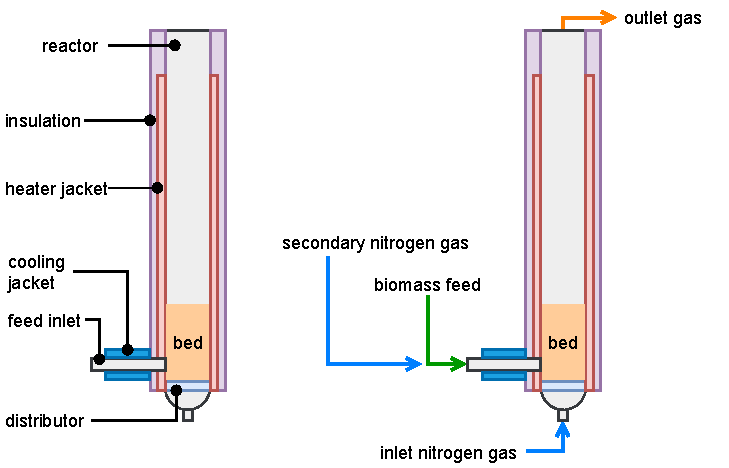
\includegraphics[width=0.8\textwidth]{figures/pyrolyzer1.pdf}
    \caption{Components (left) and inlet/outlet flows (right) of the NREL bubbling fluidized bed pyrolysis reactor.}
    \label{fig:pyrolyzer1}
\end{figure}

Dimensions for the reactor tube, feed inlet, insulation, heat jacket, and distributor plate are given in Figure \ref{fig:pyrolyzer2} and Table \ref{tab:dimensions}. The main reactor tube is a 2-inch Schedule 40 pipe; therefore, the inner and outer reactor diameters are determined from nominal pipe size tables. The gas distributor contains 18 holes in a triangular pattern \cite{French-2019}.

Typical operating conditions of the pyrolyzer are presented in Table \ref{tab:operating}. Pressure drop across the distributor is about 80-90 inches of H$_2$O. Nitrogen gas is used to fluidize the bed and assist biomass particles through the feed inlet tube. Experiments are conducted with an initial mass of sand in the bed; sand is not fed into the reactor during operation. Insulation surrounds the reactor while heat jackets extend almost the entire height of the unit. A cooling jacket surrounds the feed inlet tube. Pyrolysis vapors exit directly out the top of the reactor via a straight tube \cite{French-2019}.

\begin{figure}[H]
    \centering
    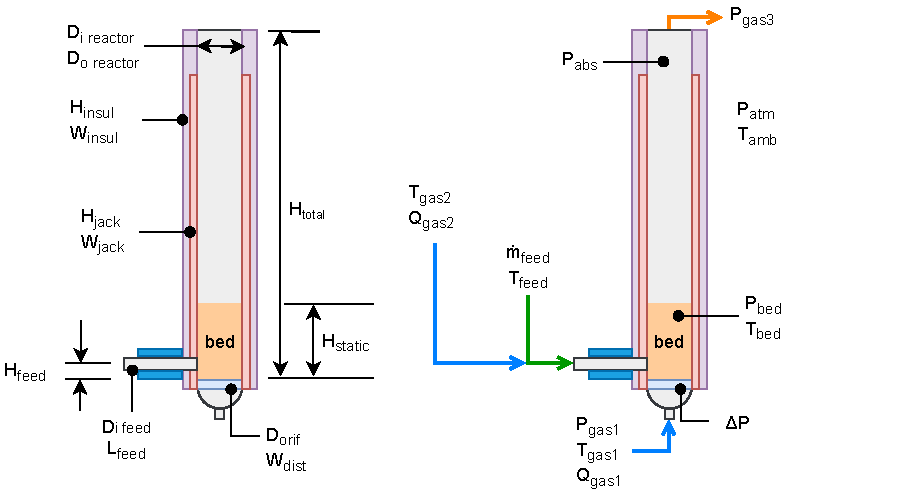
\includegraphics[width=\textwidth]{figures/pyrolyzer2.pdf}
    \caption{Dimensions and typical fast pyrolysis operating conditions for the NREL 2FBR pyrolyzer reactor.}
    \label{fig:pyrolyzer2}
\end{figure}

\begin{table}[H]
    \centering
    \caption{Dimensions for components of the fluidized bed pyrolysis reactor.}
    \label{tab:dimensions}
    \begin{tabular}{llrl}
        \toprule
        Reactor dimension & Symbol & Value & Units \\
        \midrule
        Inner reactor diameter              & D$_{\textrm{i, reactor}}$  & 5.25  & cm \\
        Outer reactor diameter              & D$_{\textrm{o, reactor}}$  & 6.03  & cm \\
        Static bed height                   & H$_{\textrm{static}}$      & 10.16 & cm \\
        Total reactor height                & H$_{\textrm{total}}$       & 43.18 & cm \\
        Feed inlet inner diameter           & D$_{\textrm{i, feed}}$     & 1.27  & cm \\
        Feed height from top of distributor & H$_{\textrm{feed}}$        & 1.9   & cm \\
        Feed inlet tube length              & L$_{\textrm{feed}}$        & 18.29 & cm \\
        Insulation height                   & H$_{\textrm{insul}}$       & 43.18 & cm \\
        Insulation thickness                & W$_{\textrm{insul}}$       & 10    & cm \\
        Jacket height                       & H$_{\textrm{jack}}$        & 35    & cm \\
        Jacket thickness                    & W$_{\textrm{jack}}$        & 5     & cm \\
        Diameter of distributor orifices    & D$_{\textrm{orif}}$        & 0.08  & cm \\
        Thickness of distributor plate      & W$_{\textrm{dist}}$        & 3.17  & mm \\
        Number of orifices in distributor   & n                          & 18    & -- \\
        \bottomrule
    \end{tabular}
\end{table}

\begin{table}[H]
    \centering
    \caption{Typical operating conditions for the fluidized bed pyrolysis reactor. Atmospheric pressure considers elevation of NREL site in Golden, CO.}
    \label{tab:operating}
    \begin{tabular}{llrl}
        \toprule
        Reactor condition & Symbol & Value & Units \\
        \midrule
        Absolute pressure in reactor   & P$_{\textrm{abs}}$  & 101.3     & kPa \\
        Atmospheric pressure           & P$_{\textrm{atm}}$  & 81        & kPa \\
        Ambient air temperature        & T$_{\textrm{amb}}$  & 300.15    & K \\
        Absolute bed pressure          & P$_{\textrm{bed}}$  & 115       & kPa  \\
        Bed temperature                & T$_{\textrm{bed}}$  & 773.15    & K \\
        Pressure drop over distributor & $\Delta$ P          & 21.17     & KPa \\
        Absolute inlet gas pressure    & P$_{\textrm{gas1}}$ & 110--140  & kPa \\
        Inlet gas temperature          & T$_{\textrm{gas1}}$ & 773.15    & K \\
        Inlet gas flowrate             & Q$_{\textrm{gas1}}$ & 14        & SLM (0.29 g/s) \\
        Secondary gas temperature      & T$_{\textrm{gas2}}$ & 298.15    & K \\
        Secondary gas flowrate         & Q$_{\textrm{gas2}}$ & 1.4       & SLM (0.029 g/s) \\
        Absolute outlet gas pressure   & P$_{\textrm{gas3}}$ & 90--110   & kPa \\
        Biomass inlet feedrate         & $\dot{{\textrm{m}}}_{\textrm{feed}}$ & 420 & g/hr \\
        Biomass inlet temperature      & T$_{\textrm{feed}}$ & 298.15    & K \\
        \bottomrule
    \end{tabular}
\end{table}

\subsection{Feedstock proximate and ultimate analyses}

Proximate and ultimate analysis measurements for each feedstock are given in Tables \ref{tab:proximate} and \ref{tab:ultimate} on an as-determined basis (ad). A visual comparison of the proximate and ultimate analysis measurements is shown in Figure \ref{fig:prox-ult-analysis}. Overall, the elemental composition of each feedstock is similar based on the ultimate analysis data. Differences in elemental fractions occur mainly in the C and O fractions with a maximum difference of approximately 3 wt.\% and 5 wt.\% respectively. For the proximate analysis fractions, the largest differences are observed for the fixed carbon (FC) and volatile matter (VM) at 10 wt.\% and 13 wt.\% respectively. A maximum difference of about 3 wt.\% is seen for the ash and moisture fractions.

\begin{table}[H]
    \caption{Proximate analysis measurements given as wt. \% as-determined basis.}
    \label{tab:proximate}
    \centering
    \begin{tabular}{lcrrrrr}
        \toprule
        Name & Cycle & FC & VM & Ash & Moisture & Total \\
        \midrule
        Residues                    & 1  & 20.72 & 72.92 & 1.45 & 4.92 & 100.01 \\
        Stem wood                   & 2  & 16.79 & 79.40 & 0.28 & 3.55 & 100.02 \\
        Bark                        & 3  & 27.16 & 66.29 & 0.70 & 5.86 & 100.01 \\
        Needles                     & 4  & 23.26 & 69.54 & 3.78 & 3.42 & 100.00 \\
        Bark + needles              & 5  & 24.35 & 68.30 & 2.52 & 4.85 & 100.02 \\
        Residues (rep 1)            & 8  & 20.78 & 72.37 & 1.65 & 5.20 & 100.00 \\
        Residues:bark:needles 1:1:1 & 10 & 23.75 & 69.02 & 2.05 & 5.19 & 100.01 \\
        Residues:bark:needles 1:2:2 & 11 & 24.12 & 68.57 & 2.02 & 5.29 & 100.00 \\
        Air classified (10 Hz)      & 12 & 19.92 & 75.59 & 0.92 & 3.57 & 100.00 \\
        Air classified (28 Hz)      & 13 & 18.68 & 76.31 & 0.61 & 4.41 & 100.01 \\
        Whole tree (13 yr)          & 15 & 19.15 & 76.72 & 0.44 & 3.71 & 100.02 \\
        Stem wood (13 yr)           & 16 & 18.60 & 78.37 & 0.30 & 2.75 & 100.02 \\
        \cmidrule{3-6}
        \multicolumn{2}{l}{Maximum difference} & 10.37 & 13.11 & 3.50 & 3.11 & \\
        \bottomrule
    \end{tabular}
\end{table}

\begin{table}[H]
    \caption{Ultimate analysis measurements given as wt. \% as-determined basis.}
    \label{tab:ultimate}
    \centering
    \begin{tabular}{lcrrrrrr}
        \toprule
        Name & Cycle & C & H & O & N & S & Total \\
        \midrule
        Residues                    & 1  & 49.63 & 6.52 & 41.87 & 0.49 & 0.04 & 98.55 \\
        Stem wood                   & 2  & 48.89 & 6.53 & 44.12 & 0.18 & 0.01 & 99.73 \\
        Bark                        & 3  & 51.84 & 6.14 & 40.97 & 0.34 & 0.02 & 99.31 \\
        Needles                     & 4  & 50.22 & 6.22 & 38.77 & 0.92 & 0.09 & 96.22 \\
        Bark + needles              & 5  & 50.35 & 6.18 & 40.21 & 0.67 & 0.06 & 97.47 \\
        Residues (rep 1)            & 8  & 49.82 & 6.56 & 41.34 & 0.58 & 0.05 & 98.35 \\
        Residues:bark:needles 1:1:1 & 10 & 50.58 & 6.31 & 40.43 & 0.59 & 0.05 & 97.96 \\
        Residues:bark:needles 1:2:2 & 11 & 50.86 & 6.24 & 40.24 & 0.58 & 0.06 & 97.98 \\
        Air classified (10 Hz)      & 12 & 50.16 & 6.46 & 42.06 & 0.37 & 0.03 & 99.08 \\
        Air classified (28 Hz)      & 13 & 48.93 & 6.42 & 43.77 & 0.26 & 0.02 & 99.40 \\
        Whole tree (13 yr)          & 15 & 49.32 & 6.44 & 43.48 & 0.30 & 0.02 & 99.56 \\
        Stem wood (13 yr)           & 16 & 49.40 & 6.41 & 43.68 & 0.21 & 0.01 & 99.71 \\
        \cmidrule{3-7}
        \multicolumn{2}{l}{Maximum difference} & 2.95 & 0.42 & 5.35 & 0.74 & 0.08 & \\
        \bottomrule
    \end{tabular}
\end{table}

\begin{figure}[H]
    \centering
    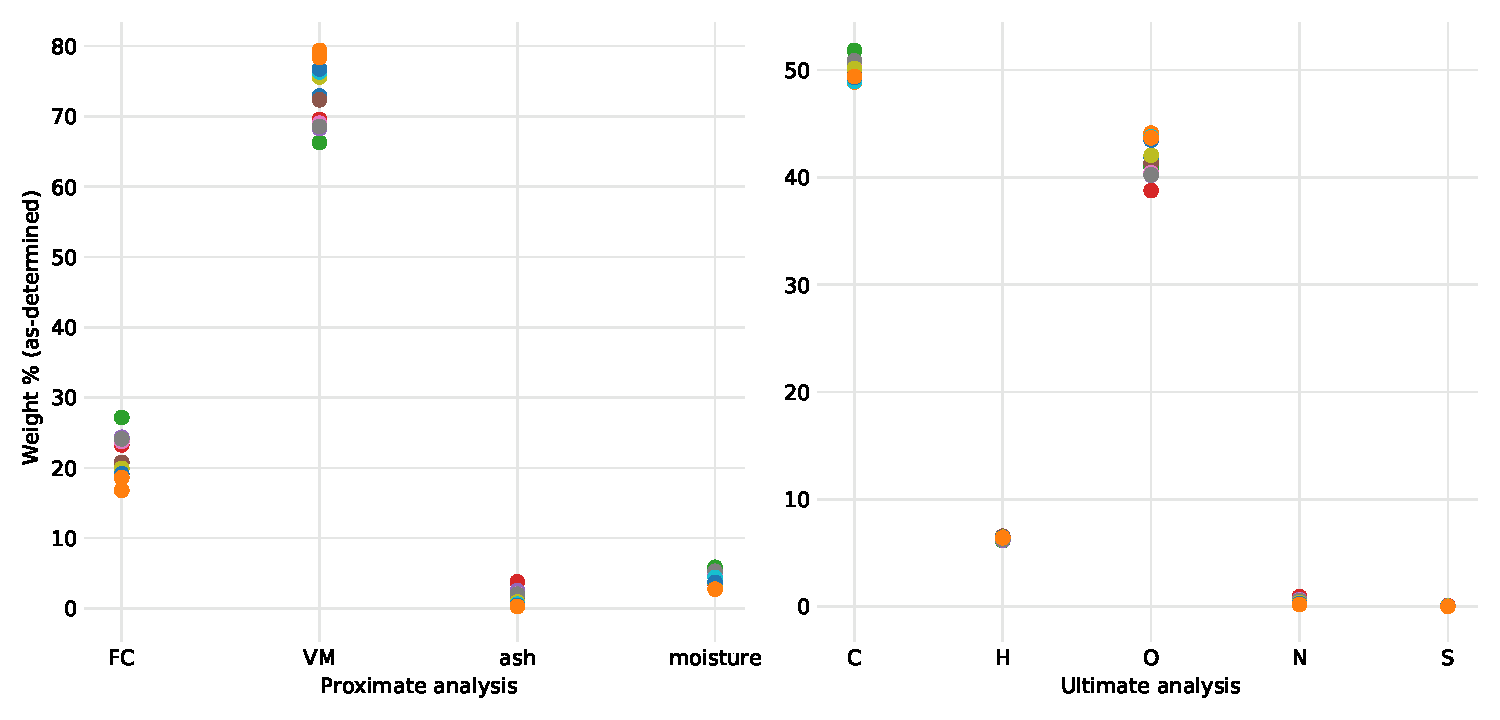
\includegraphics[width=\textwidth]{figures/prox-ult-analysis.pdf}
    \caption{Comparison of proximate (left) and ultimate (right) analysis measurements for each feedstock. Values represent wt. \% as-determined basis.}
    \label{fig:prox-ult-analysis}
\end{figure}

The proximate analysis data was converted to different bases using ASTM methods \cite{Astm-2015}. Equations \ref{eq:prox-bases1}--\ref{eq:prox-bases4} convert the as-determined (ad) basis to as-received (ar), dry (d), and dry ash-free (daf) bases where $X$ is the wt. \% of the corresponding basis value, $M$ is the moisture content, and $ADL$ is the air-dry loss assumed to be 22 wt. \%. As an example, to obtain the as-received value of the fixed carbon use $FC_{ar} = FC_{ad} \times \frac{100 - M_{ar}}{100 - M_{ad}}$.

\begin{align}
    M_{ar} &= \left(M_{ad} \times \frac{100 - ADL}{100}\right) + ADL \label{eq:prox-bases1} \\
    X_{ar} &= X_{ad} \times \frac{100 - M_{ar}}{100 - M_{ad}} \\
    X_{d} &= X_{ad} \times \frac{100}{100 - M_{ad}} \\
    X_{daf} &= X_{ad} \times \frac{100}{100 - M_{ad} - ash_{ad}} \label{eq:prox-bases4}
\end{align}

Similarly, the ultimate analysis data was also converted to different bases using the ASTM methods \cite{Astm-2015}. Equations \ref{eq:prox-bases1}--\ref{eq:prox-bases4} convert the carbon, nitrogen, and sulfur fractions to different bases while Equations \ref{eq:ult-bases1}--\ref{eq:ult-bases4} are for the hydrogen and oxygen fractions. Equation \ref{eq:cho-basis} calculates the CHO basis from the dry ash-free basis.

\begin{align}
    H_{ar} &= (H_{ad} - 0.1119\, M_{ad}) \times \frac{100 - M_{ar}}{100 - M_{ad}} \label{eq:ult-bases1} \\
    O_{ar} &= (O_{ad} - 0.8881\, M_{ad}) \times \frac{100 - M_{ar}}{100 - M_{ad}} \\
    H_{d} &= (H_{ad} - 0.1119\, M_{ad}) \times \frac{100}{100 - M_{ad}} \\
    O_{d} &= (O_{ad} - 0.8881\, M_{ad}) \times \frac{100}{100 - M_{ad}} \label{eq:ult-bases4} \\
    X_{cho} &= X_{daf} \times \frac{100}{100 - N_{daf} - S_{daf}} \label{eq:cho-basis}
\end{align}

Table \ref{tab:basis} presents the proximate and ultimate analysis data on an as-determined (ad), as-received (ar), dry (d), dry ash-free (daf), and CHO basis. The reported H and O for the ultimate analysis data does not include the H and O in the moisture; therefore, the total value for the as-determined basis excludes the moisture percentage for the ultimate analysis.

\newpage
\begin{longtable}{lrrrrr}
    \caption{Proximate and ultimate analysis basis values for each feedstock given as wt. \%. Reported H and O values for ultimate analysis ad-basis excludes H and O in moisture.}
    \label{tab:basis} \\

    \textbf{Residues} & ad & ar & d & daf & cho \\
    \hline \\
    FC       & 20.72  & 17.33  & 21.79  & 22.13  & -- \\
    VM       & 72.92  & 60.99  & 76.69  & 77.88  & -- \\
    ash      & 1.45   & 1.21   & 1.53   & --     & -- \\
    moisture & 4.92   & 20.58  & --     & --     & -- \\
    total    & 100.01 & 100.01 & 100.01 & 100.01 & -- \\
    \\
    C        & 49.63  & 38.71 & 52.20 & 53.01 & 53.31 \\
    H        & 6.52   & 4.66  & 6.28  & 6.38  & 6.41 \\
    O        & 41.87  & 29.25 & 39.44 & 40.05 & 40.28 \\
    N        & 0.49   & 0.38  & 0.52  & 0.52  & -- \\
    S        & 0.04   & 0.03  & 0.04  & 0.04  & -- \\
    ash      & 1.45   & 1.13  & 1.53  & --    & -- \\
    moisture & (4.92) & 25.84 & --    & --    & -- \\
    total    & 100    & 100   & 100   & 100   & 100 \\
    \\

    \textbf{Stem wood} & ad & ar & d & daf & cho \\
    \hline \\
    FC       & 16.79  & 13.10  & 17.41  & 17.46  & -- \\
    VM       & 79.40  & 61.93  & 82.32  & 82.56  & -- \\
    ash      & 0.28   & 0.22   & 0.29   & --     & -- \\
    moisture & 3.55   & 24.77  & --     & --     & -- \\
    total    & 100.02 & 100.02 & 100.02 & 100.02 & -- \\
    \\
    C        & 48.89  & 38.13  & 50.69  & 50.84  & 50.94 \\
    H        & 6.53   & 4.78   & 6.36   & 6.38   & 6.39 \\
    O        & 44.12  & 31.95  & 42.48  & 42.60  & 42.68 \\
    N        & 0.18   & 0.14   & 0.19   & 0.19   & -- \\
    S        & 0.01   & 0.01   & 0.01   & 0.01   & -- \\
    ash      & 0.28   & 0.22   & 0.29   & --     & -- \\
    moisture & (3.55) & 24.77  & --     & --     & -- \\
    total    & 100.01 & 100.01 & 100.01 & 100.01 & 100.01 \\
    \\

    \textbf{Bark} & ad & ar & d & daf & cho \\
    \hline \\
    FC       & 27.16  & 21.18  & 28.85  & 29.07  & -- \\
    VM       & 66.29  & 51.71  & 70.42  & 70.94  & -- \\
    ash      & 0.70   & 0.55   & 0.74   & --     & -- \\
    moisture & 5.86   & 26.57  & --     & --     & -- \\
    total    & 100.01 & 100.01 & 100.01 & 100.01 & -- \\
    \\
    C        & 51.84  & 40.44  & 55.07  & 55.48  & 55.69 \\
    H        & 6.14   & 4.28   & 5.83   & 5.87   & 5.89 \\
    O        & 40.97  & 27.90  & 37.99  & 38.28  & 38.42 \\
    N        & 0.34   & 0.27   & 0.36   & 0.36   & -- \\
    S        & 0.02   & 0.02   & 0.02   & 0.02   & -- \\
    ash      & 0.70   & 0.55   & 0.74   & --     & -- \\
    moisture & (5.86) & 26.57  & --     & --     & -- \\
    total    & 100.01 & 100.01 & 100.01 & 100.01 & 100.01 \\
    \\

    \textbf{Needles} & ad & ar & d & daf & cho \\
    \hline \\
    FC       & 23.26  & 18.14  & 24.08  & 25.06  & -- \\
    VM       & 69.54  & 54.24  & 72.00  & 74.94  & -- \\
    ash      & 3.78   & 2.95   & 3.91   & --     & -- \\
    moisture & 3.42   & 24.67  & --     & --     & -- \\
    total    & 100    & 100    & 100    & 100    & -- \\
    \\
    C        & 50.22  & 39.17  & 52.00  & 54.12  & 54.71 \\
    H        & 6.22   & 4.55   & 6.04   & 6.29   & 6.36 \\
    O        & 38.77  & 27.87  & 37.00  & 38.51  & 38.93 \\
    N        & 0.92   & 0.72   & 0.95   & 0.99   & -- \\
    S        & 0.09   & 0.07   & 0.09   & 0.10   & -- \\
    ash      & 3.78   & 2.95   & 3.91   & --     & -- \\
    moisture & (3.42) & 24.67  & --     & --     & -- \\
    total    & 100    & 100    & 100    & 100    & 100 \\
    \\

    \textbf{Bark + needles} & ad & ar & d & daf & cho \\
    \hline \\
    FC       & 24.35  & 18.99  & 25.59  & 26.29  & -- \\
    VM       & 68.30  & 53.27  & 71.78  & 73.73  & -- \\
    ash      & 2.52   & 1.97   & 2.65   & --     & -- \\
    moisture & 4.85   & 25.78  & --     & --     & -- \\
    total    & 100.02 & 100.02 & 100.02 & 10.02  & -- \\
    \\
    C        & 50.35  & 39.27  & 52.92  & 54.36  & 54.79 \\
    H        & 6.18   & 4.40   & 5.92   & 6.09   & 6.13 \\
    O        & 40.21  & 28.00  & 37.73  & 38.76  & 39.07 \\
    N        & 0.67   & 0.52   & 0.70   & 0.72   & -- \\
    S        & 0.06   & 0.05   & 0.06   & 0.06   & -- \\
    ash      & 2.52   & 1.97   & 2.65   & --     & -- \\
    moisture & (4.85) & 25.78  & --     & --     & -- \\
    total    & 99.99  & 99.99  & 99.99  & 99.99  & 99.99 \\
    \\

    \textbf{Residues (rep 1)} & ad & ar & d & daf & cho \\
    \hline \\
    FC       & 20.78  & 16.21  & 21.92  & 22.31  & -- \\
    VM       & 72.37  & 56.45  & 76.34  & 77.69  & -- \\
    ash      & 1.65   & 1.29   & 1.74   & --     & -- \\
    moisture & 5.20   & 26.06  & --     & --     & -- \\
    total    & 100    & 100    & 100    & 100    & -- \\
    \\
    C        & 49.82  & 38.86  & 52.55  & 53.48  & 53.85 \\
    H        & 6.56   & 4.66   & 6.31   & 6.42   & 6.46 \\
    O        & 41.34  & 28.64  & 38.74  & 39.42  & 39.69 \\
    N        & 0.58   & 0.45   & 0.61   & 0.62   & -- \\
    S        & 0.05   & 0.04   & 0.05   & 0.05   & -- \\
    ash      & 1.65   & 1.29   & 1.74   & --     & -- \\
    moisture & (5.20) & 26.06  & --     & --     & -- \\
    total    & 100    & 100    & 100    & 100    & 100 \\
    \\

    \textbf{Residues:bark:needles 1:1:1} & ad & ar & d & daf & cho \\
    \hline \\
    FC       & 23.75  & 18.52  & 25.05  & 25.60  & -- \\
    VM       & 69.02  & 53.84  & 72.80  & 74.41  & -- \\
    ash      & 2.05   & 1.60   & 2.16   & --     & -- \\
    moisture & 5.19   & 26.05  & --     & --     & -- \\
    total    & 100.01 & 100.01 & 100.01 & 100.01 & -- \\
    \\
    C        & 50.58  & 39.45  & 53.35  & 54.53  & 54.91 \\
    H        & 6.31   & 4.47   & 6.04   & 6.18   & 6.22 \\
    O        & 40.43  & 27.94  & 37.78  & 38.62  & 38.88 \\
    N        & 0.59   & 0.46   & 0.62   & 0.64   & -- \\
    S        & 0.05   & 0.04   & 0.05   & 0.05   & -- \\
    ash      & 2.05   & 1.60   & 2.16   & --     & -- \\
    moisture & (5.19) & 26.05  & --     & --     & -- \\
    total    & 100.01 & 100.01 & 100.01 & 100.01 & 100.01 \\
    \\

    \textbf{Residues:bark:needles 1:2:2} & ad & ar & d & daf & cho \\
    \hline \\
    FC       & 24.12  & 18.81  & 25.47  & 26.02  & -- \\
    VM       & 68.57  & 53.48  & 72.40  & 73.98  & -- \\
    ash      & 2.02   & 1.58   & 2.13   & --     & -- \\
    moisture & 5.29   & 26.13  & --     & --     & -- \\
    total    & 100    & 100    & 100    & 100    & -- \\
    \\
    C        & 50.86  & 39.67  & 53.70  & 54.87  & 55.25 \\
    H        & 6.24   & 4.41   & 5.96   & 6.09   & 6.14 \\
    O        & 40.24  & 27.72  & 37.53  & 38.34  & 38.61 \\
    N        & 0.58   & 0.45   & 0.61   & 0.63   & -- \\
    S        & 0.06   & 0.05   & 0.06   & 0.06   & -- \\
    ash      & 2.02   & 1.58   & 2.13   & --     & -- \\
    moisture & (5.29) & 26.13  & --     & --     & -- \\
    total    & 100    & 100    & 100    & 100    & 100 \\
    \\

    \textbf{Air classified 10 Hz} & ad & ar & d & daf & cho \\
    \hline \\
    FC       & 19.92  & 15.54  & 20.66  & 20.86  & -- \\
    VM       & 75.59  & 58.96  & 78.39  & 79.14  & -- \\
    ash      & 0.92   & 0.72   & 0.95   & --     & -- \\
    moisture & 3.57   & 24.78  & --     & --     & -- \\
    total    & 100    & 100    & 100    & 100    & -- \\
    \\
    C        & 50.16  & 39.12  & 52.02  & 52.52  & 52.74 \\
    H        & 6.46   & 4.73   & 6.28   & 6.35   & 6.37 \\
    O        & 42.06  & 30.33  & 40.33  & 40.72  & 40.89 \\
    N        & 0.37   & 0.29   & 0.38   & 0.39   & -- \\
    S        & 0.03   & 0.02   & 0.03   & 0.03   & -- \\
    ash      & 0.92   & 0.72   & 0.95   & --     & -- \\
    moisture & (3.57) & 24.78  & --     & --     & -- \\
    total    & 100    & 100    & 100    & 100    & 100 \\
    \\

    \textbf{Air classified 28 Hz} & ad & ar & d & daf & cho \\
    \hline \\
    FC       & 18.68  & 14.57  & 19.54  & 19.67  & -- \\
    VM       & 76.31  & 59.52  & 79.83  & 80.34  & -- \\
    ash      & 0.61   & 0.48   & 0.64   & --     & -- \\
    moisture & 4.41   & 25.44  & --     & --     & -- \\
    total    & 100.01 & 100.01 & 100.01 & 100.01 & -- \\
    \\
    C        & 48.93  & 38.17  & 51.19  & 51.52  & 51.67 \\
    H        & 6.42   & 4.62   & 6.20   & 6.24   & 6.26 \\
    O        & 43.77  & 31.09  & 41.69  & 41.96  & 42.08 \\
    N        & 0.26   & 0.20   & 0.27   & 0.27   & -- \\
    S        & 0.02   & 0.02   & 0.02   & 0.02   & -- \\
    ash      & 0.61   & 0.48   & 0.64   & --     & -- \\
    moisture & (4.41) & 25.44  & --     & --     & -- \\
    total    & 100.01 & 100.01 & 100.01 & 100.01 & 100.01 \\
    \\

    \textbf{Whole tree 13 yr} & ad & ar & d & daf & cho \\
    \hline \\
    FC       & 19.15  & 14.94  & 19.89  & 19.98  & -- \\
    VM       & 76.72  & 59.84  & 79.68  & 80.04  & -- \\
    ash      & 0.44   & 0.34   & 0.46   & --     & -- \\
    moisture & 3.71   & 24.89  & --     & --     & -- \\
    total    & 100.02 & 100.02 & 100.02 & 100.02 & -- \\
    \\
    C        & 49.32  & 38.47  & 51.22  & 51.46  & 51.63 \\
    H        & 6.44   & 4.70   & 6.26   & 6.29   & 6.31 \\
    O        & 43.48  & 31.34  & 41.73  & 41.93  & 42.07 \\
    N        & 0.30   & 0.23   & 0.31   & 0.31   & -- \\
    S        & 0.02   & 0.02   & 0.02   & 0.02   & -- \\
    ash      & 0.44   & 0.34   & 0.46   & --     & -- \\
    moisture & (3.71) & 24.89  & --     & --     & -- \\
    total    & 100    & 100    & 100    & 100    & 100 \\
    \\

    \textbf{Stem wood 13 yr} & ad & ar & d & daf & cho \\
    \hline \\
    FC       & 18.60  & 14.51  & 19.13  & 19.19  & -- \\
    VM       & 78.37  & 61.13  & 80.59  & 80.84  & -- \\
    ash      & 0.30   & 0.23   & 0.31   & --     & -- \\
    moisture & 2.75   & 24.14  & --     & --     & -- \\
    total    & 100.02 & 100.02 & 100.02 & 100.02 & -- \\
    \\
    C        & 49.40  & 38.53  & 50.80  & 50.95  & 51.07 \\
    H        & 6.41   & 4.76   & 6.27   & 6.29   & 6.31 \\
    O        & 43.68  & 32.17  & 42.40  & 42.54  & 42.63 \\
    N        & 0.21   & 0.16   & 0.22   & 0.22   & -- \\
    S        & 0.01   & 0.01   & 0.01   & 0.01   & -- \\
    ash      & 0.30   & 0.23   & 0.31   & --     & -- \\
    moisture & (2.75) & 24.14  & --     & --     & -- \\
    total    & 100.01 & 100.01 & 100.01 & 100.01 & 100.01 \\
\end{longtable}

\subsection{Feedstock chemical analysis}

Chemical analysis data for each feedstock was supplied by INL on a wt. \% dry basis (d). The dry basis values $P_d$ are converted to a dry ash-free basis $P_{daf}$ using Equation \ref{eq:chem-daf} where $P_{s.\,inorg.}$ is the structural inorganics and $P_{ns.\,inorg.}$ is the non-structural inorganics. A summary of the chemical analysis data and converted values are presented in Table \ref{tab:chemical} while a comparison of the as-determined values are shown in Figure \ref{fig:chem-analysis}. The largest variations in the measured chemical fractions occur for the lignin and glucan with a maximum difference of 15 wt. \% and 17.5 wt. \% respectively.

\begin{equation}
    \label{eq:chem-daf}
    P_{daf} = P_d \times \frac{100}{\sum P_d - P_{s.\,inorg.} - P_{ns.\,inorg.}}
\end{equation}

\begin{longtable}{lrr}
    \caption{Chemical analysis values shown as weight percent (wt. \%) for dry (d) and dry ash-free (daf) bases.}
    \label{tab:chemical} \\

    \textbf{Residues, Cycle 1} & d & daf \\
    \midrule
    structural inorganics     & 0.94  & -- \\
    non-structural inorganics & 0.37  & -- \\
    water extractives         & 4.91  & 5.05 \\
    ethanol extractives       & 0.62  & 0.64 \\
    acetone extractives       & 6.6   & 6.79 \\
    lignin                    & 35.52 & 36.53 \\
    glucan                    & 28.18 & 28.98 \\
    xylan                     & 7.33  & 7.54 \\
    galactan                  & 3.56  & 3.66 \\
    arabinan                  & 1.93  & 1.98 \\
    mannan                    & 7.64  & 7.86 \\
    acetyl                    & 0.95  & 0.98 \\
    total                     & 98.55 & 100 \\
    \\

    \textbf{Stem wood, Cycle 2} & d & daf \\
    \midrule
    structural inorganics     & 0.32   & -- \\
    non-structural inorganics & 0      & -- \\
    water extractives         & 2.76   & 2.72 \\
    ethanol extractives       & 0.31   & 0.31 \\
    acetone extractives       & 2.57   & 2.54 \\
    lignin                    & 30.7   & 30.29 \\
    glucan                    & 39.84  & 39.31 \\
    xylan                     & 6.3    & 6.22 \\
    galactan                  & 2.59   & 2.56 \\
    arabinan                  & 0      & 0 \\
    mannan                    & 14.94  & 14.74 \\
    acetyl                    & 1.35   & 1.33 \\
    total                     & 101.68 & 100 \\
    \\

    \textbf{Bark, Cycle 3} & d & daf \\
    \midrule
    structural inorganics     & 0.5    & -- \\
    non-structural inorganics & 0.08   & -- \\
    water extractives         & 2.9    & 2.90 \\
    ethanol extractives       & 0.46   & 0.46 \\
    acetone extractives       & 3.33   & 3.33 \\
    lignin                    & 34.34  & 34.29 \\
    glucan                    & 33.83  & 33.78 \\
    xylan                     & 7.74   & 7.73 \\
    galactan                  & 3.68   & 3.67 \\
    arabinan                  & 3.5    & 3.50 \\
    mannan                    & 9.15   & 9.14 \\
    acetyl                    & 1.21   & 1.21 \\
    total                     & 100.72 & 100 \\
    \\

    \textbf{Needles, Cycle 4} & d & daf \\
    \midrule
    structural inorganics     & 3.23  & -- \\
    non-structural inorganics & 0.56  & -- \\
    water extractives         & 5.95  & 6.29 \\
    ethanol extractives       & 1.35  & 1.43 \\
    acetone extractives       & 7.35  & 7.77 \\
    lignin                    & 41.03 & 43.35 \\
    glucan                    & 22.33 & 23.59 \\
    xylan                     & 4.12  & 4.35 \\
    galactan                  & 2.57  & 2.72 \\
    arabinan                  & 1.52  & 1.61 \\
    mannan                    & 7.44  & 7.86 \\
    acetyl                    & 0.98  & 1.04 \\
    total                     & 98.43 & 100 \\
    \\

    \textbf{Bark + needles, Cycle 5} & d & daf \\
    \midrule
    structural inorganics     & 1.76  & -- \\
    non-structural inorganics & 0.66  & -- \\
    water extractives         & 4.01  & 4.21 \\
    ethanol extractives       & 0.98  & 1.03 \\
    acetone extractives       & 5.53  & 5.81 \\
    lignin                    & 45.88 & 48.21 \\
    glucan                    & 22.75 & 23.91 \\
    xylan                     & 4.17  & 4.38 \\
    galactan                  & 3.28  & 3.45 \\
    arabinan                  & 2.4   & 2.52 \\
    mannan                    & 5.35  & 5.62 \\
    acetyl                    & 0.81  & 0.85 \\
    total                     & 97.58 & 100 \\
    \\

    \textbf{Residues (rep 1), Cycle 8} & d & daf \\
    \midrule
    structural inorganics     & 1.24  & -- \\
    non-structural inorganics & 0.19  & -- \\
    water extractives         & 6.18  & 6.40 \\
    ethanol extractives       & 0.68  & 0.70 \\
    acetone extractives       & 7.88  & 8.16 \\
    lignin                    & 35.22 & 36.49 \\
    glucan                    & 26.48 & 27.44 \\
    xylan                     & 6.52  & 6.76 \\
    galactan                  & 3.44  & 3.56 \\
    arabinan                  & 2.84  & 2.94 \\
    mannan                    & 6.33  & 6.56 \\
    acetyl                    & 0.94  & 0.97 \\
    total                     & 97.94 & 100 \\
    \\

    \textbf{Residues:bark:needles 1:1:1, Cycle 10} & d & daf \\
    \midrule
    structural inorganics     & 1.66  & -- \\
    non-structural inorganics & 0.02  & -- \\
    water extractives         & 5.76  & 5.93 \\
    ethanol extractives       & 1.02  & 1.05 \\
    acetone extractives       & 6.87  & 7.07 \\
    lignin                    & 42.06 & 43.28 \\
    glucan                    & 23.37 & 24.05 \\
    xylan                     & 5.07  & 5.22 \\
    galactan                  & 2.95  & 3.04 \\
    arabinan                  & 1.62  & 1.67 \\
    mannan                    & 7.55  & 7.77 \\
    acetyl                    & 0.9   & 0.93 \\
    total                     & 98.85 & 100 \\
    \\

    \textbf{Residues:bark:needles 1:2:2, Cycle 11} & d & daf \\
    \midrule
    structural inorganics     & 1.91  & -- \\
    non-structural inorganics & 0.21  & -- \\
    water extractives         & 5.53  & 5.79 \\
    ethanol extractives       & 1.04  & 1.09 \\
    acetone extractives       & 6.51  & 6.81 \\
    lignin                    & 42.9  & 44.89 \\
    glucan                    & 22.92 & 23.98 \\
    xylan                     & 4.64  & 4.86 \\
    galactan                  & 3.03  & 3.17 \\
    arabinan                  & 2.23  & 2.33 \\
    mannan                    & 5.91  & 6.18 \\
    acetyl                    & 0.85  & 0.89 \\
    total                     & 97.68 & 100 \\
    \\

    \textbf{Air classified (10 Hz), Cycle 12} & d & daf \\
    \midrule
    structural inorganics     & 0.55  & -- \\
    non-structural inorganics & 0.31  & -- \\
    water extractives         & 3.26  & 3.31 \\
    ethanol extractives       & 0.44  & 0.45 \\
    acetone extractives       & 4.02  & 4.08 \\
    lignin                    & 35.11 & 35.60 \\
    glucan                    & 31.99 & 32.44 \\
    xylan                     & 7.63  & 7.74 \\
    galactan                  & 3.63  & 3.68 \\
    arabinan                  & 1.34  & 1.36 \\
    mannan                    & 10.01 & 10.15 \\
    acetyl                    & 1.18  & 1.20 \\
    total                     & 99.47 & 100 \\
    \\

    \textbf{Air classified (28 Hz), Cycle 13} & d & daf \\
    \midrule
    structural inorganics     & 0.38   & -- \\
    non-structural inorganics & 0.22   & -- \\
    water extractives         & 1.76   & 1.76 \\
    ethanol extractives       & 0.31   & 0.31 \\
    acetone extractives       & 2.4    & 2.40 \\
    lignin                    & 35.23  & 35.23 \\
    glucan                    & 34.37  & 34.37 \\
    xylan                     & 8.39   & 8.39 \\
    galactan                  & 3.9    & 3.90 \\
    arabinan                  & 0      & 0 \\
    mannan                    & 12.41  & 12.41 \\
    acetyl                    & 1.24   & 1.24 \\
    total                     & 100.61 & 100 \\
    \\

    \textbf{Whole tree (13 yr), Cycle 15} & d & daf \\
    \midrule
    structural inorganics     & 0.5   & -- \\
    non-structural inorganics & 0.08  & -- \\
    water extractives         & 2.9   & 2.93 \\
    ethanol extractives       & 0.46  & 0.46 \\
    acetone extractives       & 3.33  & 3.36 \\
    lignin                    & 33.34 & 33.63 \\
    glucan                    & 33.83 & 34.12 \\
    xylan                     & 7.74  & 7.81 \\
    galactan                  & 3.68  & 3.71 \\
    arabinan                  & 3.5   & 3.53 \\
    mannan                    & 9.15  & 9.23 \\
    acetyl                    & 1.21  & 1.22 \\
    total                     & 99.72 & 100 \\
    \\

    \textbf{Stem wood (13 yr), Cycle 16} & d & daf \\
    \midrule
    structural inorganics     & 0.32   & -- \\
    non-structural inorganics & 0      & -- \\
    water extractives         & 1.56   & 1.53 \\
    ethanol extractives       & 0.34   & 0.33 \\
    acetone extractives       & 1.76   & 1.73 \\
    lignin                    & 33.4   & 32.80 \\
    glucan                    & 38.15  & 37.46 \\
    xylan                     & 7.97   & 7.83 \\
    galactan                  & 3.63   & 3.56 \\
    arabinan                  & 3.53   & 3.47 \\
    mannan                    & 10.08  & 9.90 \\
    acetyl                    & 1.41   & 1.38 \\
    total                     & 102.15 & 100 \\
\end{longtable}

\begin{figure}[H]
    \centering
    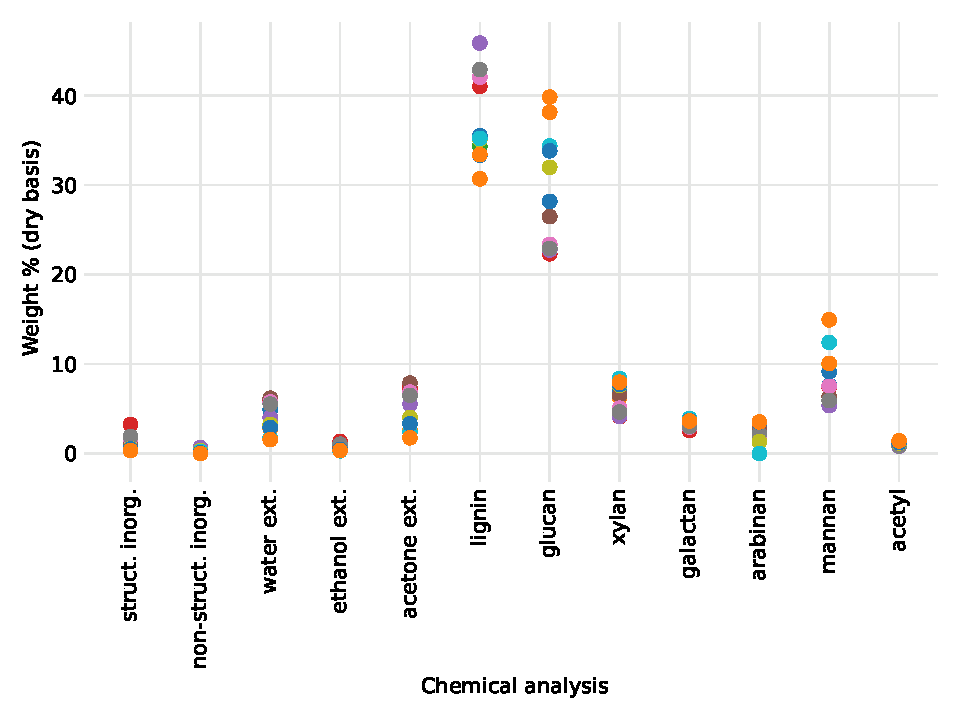
\includegraphics[width=0.8\textwidth]{figures/chem-analysis.pdf}
    \caption{Comparison of chemical analysis measurements for each feedstock.}
    \label{fig:chem-analysis}
\end{figure}

\subsection{Bed particle characteristics}

Characteristics of the sand particles that represent the fluidized bed material were obtained by NETL and are summarized in Table \ref{tab:sand}. A microscope image of the sand particles is shown in Figure \ref{fig:sand}. The particle density was determined from a helium pycnometer while size distribution and sphericity was obtained from QICPIC image analysis \cite{Netl-2021}. At the time of writing this report, bed particle characteristics were not utilized in the reactor models discussed in subsequent sections.

\begin{table}[H]
    \caption{Bed material (sand) characteristics.}
    \label{tab:sand}
    \centering
    \begin{tabular}{lcrl}
        \toprule
        Parameter & Symbol & Value & Units \\
        \midrule
        Particle envelope density     & $\rho$ & 2.7051 & g/cm$^3$ \\
        Standard deviation of density & --     & 0.0004 & g/cm$^3$ \\
        Sauter mean diameter          & SMD    & 509    & $\mu$m \\
        Average particle sphericity   & $\phi$ & 0.874  & -- \\
        \bottomrule
    \end{tabular}
\end{table}

\begin{figure}[H]
    \centering
    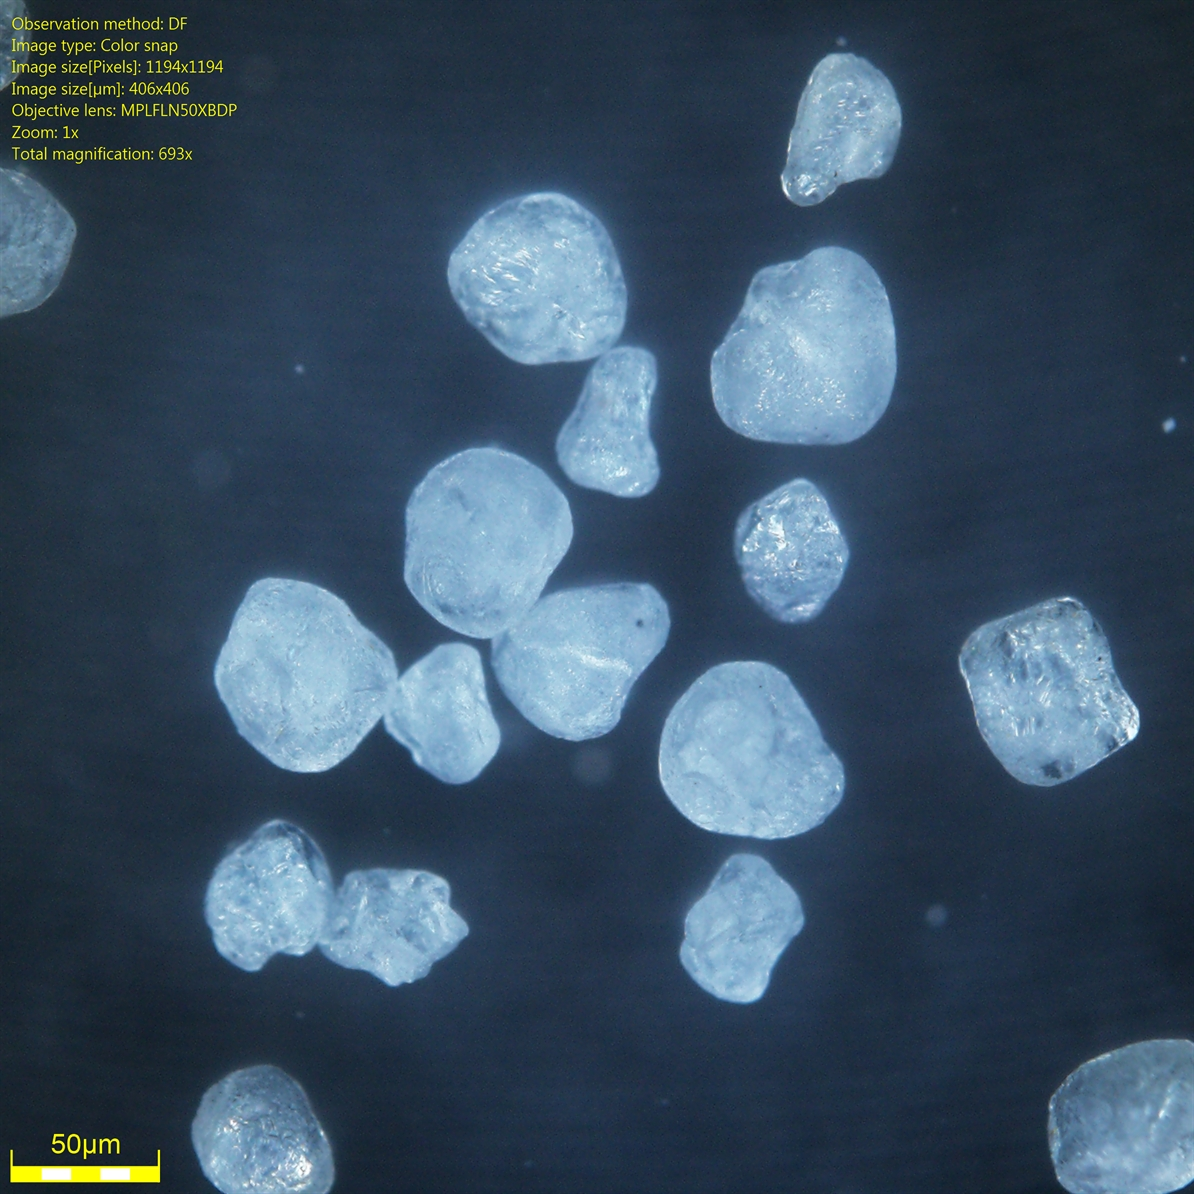
\includegraphics[width=0.5\textwidth]{figures/sand.jpg}
    \caption{Microscope image of sand particles used for the bed material.}
    \label{fig:sand}
\end{figure}

\subsection{Product yields}

Product yields measured from the fast pyrolysis of each feedstock in the fluidized bed reactor are given in Table \ref{tab:yields}. A comparison of the product yields from each feedstock is shown in Figure \ref{fig:yields}. The oil and char yields are the most variable between the different feedstocks while condensables and water vapor differ by a few percent.

\begin{table}[H]
    \caption{Measured reactor yields from each feedstock experiment. Values expressed as percent wet basis (w).}
    \label{tab:yields}
    \centering
    \begin{tabular}{lcccccr}
        Feedstock & \rotatebox{90}{Oil} & \rotatebox{90}{Condensables} & \rotatebox{90}{Light gas} & \rotatebox{90}{Water vapor} & \rotatebox{90}{Char} & \rotatebox{90}{Total} \\
        \toprule
        Residues                    & 63.5 & 1.6 & 14.7 & 0.4 & 15.2 & 95.4 \\
        Stem wood                   & 72.3 & 2.8 & 14.1 & 1.2 & 10.9 & 101.3 \\
        Bark                        & 58.3 & 1.3 & 11.4 & 0.8 & 31.9 & 103.7 \\
        Needles                     & 55.4 & 2.7 & 14.5 & 0.6 & 25.6 & 98.8 \\
        Bark + needles              & 55.5 & 1.3 & 15.1 & 1.2 & 16.5 & 89.6 \\
        Residues (rep 1)            & 62.6 & 2.5 & 15.9 & 2.5 & 17.3 & 100.8 \\
        Residues:bark:needles 1:1:1 & 58.3 & 3.1 & 14.3 & 0.7 & 24.6 & 101.0 \\
        Residues:bark:needles 1:2:2 & 57.1 & 0.6 & 15.0 & 2.0 & 25.0 & 99.7 \\
        Air classified (10 Hz)      & 57.6 & 3.0 & 16.2 & 3.2 & 16.3 & 96.3 \\
        Air classified (28 Hz)      & 65.0 & 2.5 & 17.9 & 1.6 & 13.9 & 100.9 \\
        Whole tree (13 yr)          & 63.1 & 1.8 & 17.7 & 2.1 & 13.9 & 98.6 \\
        Stem wood (13 yr)           & 67.8 & 1.9 & 15.2 & 3.2 & 12.2 & 100.3 \\
        \bottomrule
    \end{tabular}
\end{table}

\begin{figure}[H]
    \centering
    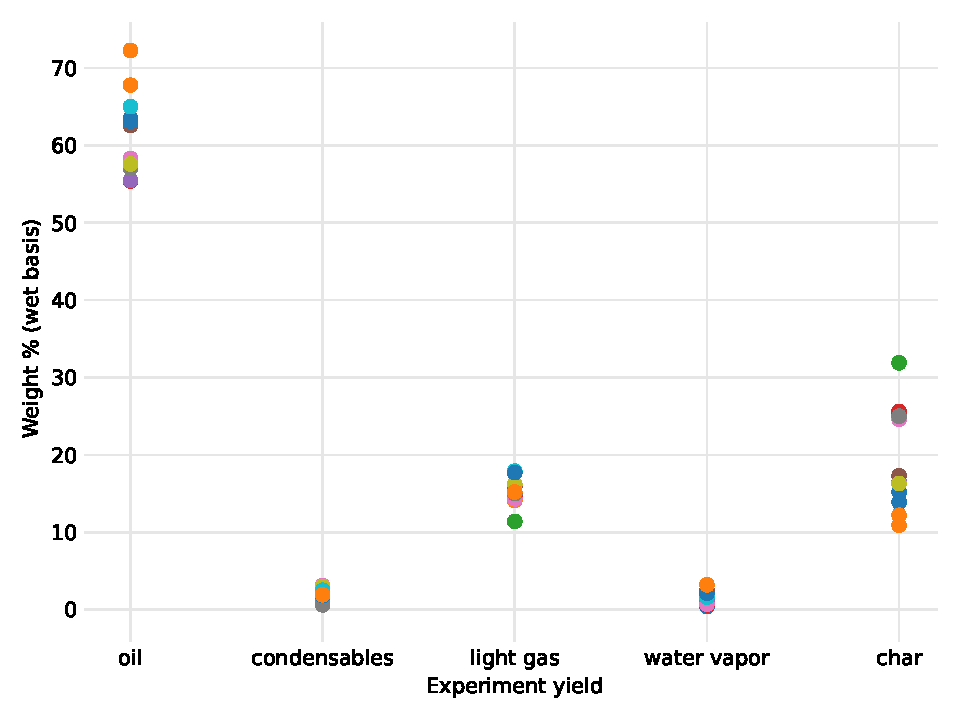
\includegraphics[width=0.8\textwidth]{figures/yields.pdf}
    \caption{Comparison of the measured product yields for each feedstock. Values shown as percent wet basis.}
    \label{fig:yields}
\end{figure}

\section{Model development}

This section details the biomass pyrolysis kinetics scheme, biomass composition characterization method, and the reduced-order reactor models.

\subsection{Biomass pyrolysis kinetics}

The kinetic reaction mechanisms presented in the Debiagi et al. 2018 paper \cite{Debiagi-2018} were used to model biomass pyrolysis in the fluidized bed reactor. Table \ref{tab:chem-kinetics} summarizes the reactions along with the associated prefactors and activation energies. A description of the chemical species in the Debiagi et al. kinetic scheme is provided in Table \ref{tab:chem-species}. Species are grouped into solid, metaplastic, gas, and liquid phases. Solid and metaplastic species are combined and compared to the reactor's char yield. All liquid species are combined and compared to the reactor's total liquid yield.

% \setlength\LTleft{-0.2in}
% \setlength\LTright{-0.2in}
\begin{center}
\footnotesize
\begin{longtable}{cp{4in}rr}
    \caption{Kinetic reactions for biomass pyrolysis where A is the prefactor, E is the activation energy, and T is temperature. Source \cite{Debiagi-2018}.}
    \label{tab:chem-kinetics} \\
    \toprule
    Item & Reaction & A (1/s) & E (cal/mol) \\
    \midrule
    1  & CELL $\rightarrow$ CELLA & 1.5 $\times$ 10$^{14}$ & 47,000 \\
    2  & CELLA $\rightarrow$ 0.40 CH2OHCHO + 0.03 CHOCHO + 0.17 CH3CHO + 0.25 C6H6O3 + 0.35 C2H5CHO + 0.20 CH3OH + 0.15 CH2O + 0.49 CO + 0.05 G\{CO\} + 0.43 CO2 + 0.13 H2 + 0.93 H2O + 0.05 G\{COH2\} loose + 0.02 HCOOH + 0.05 CH2OHCH2CHO + 0.05 CH4 + 0.1 G\{H2\} + 0.66 CHAR & 2.5 $\times$ 10$^6$ & 19,100 \\
    3  & CELLA $\rightarrow$ C6H10O5 & 3.3 $\times$ T & 10,000 \\
    4  & CELL $\rightarrow$ 4.45 H2O + 5.45 CHAR + 0.12 G\{COH2\} stiff + 0.18 G\{COH2\} loose + 0.25 G\{CO\} + 0.125 G\{H2\} + 0.125 H2 & 9.0 $\times$ 10$^7$ & 31,000 \\
    5  & GMSW $\rightarrow$ 0.70 HCE1 + 0.30 HCE2 & 1.0 $\times$ 10$^{10}$ & 31,000 \\
    6  & XYHW $\rightarrow$ 0.35 HCE1 + 0.65 HCE2 & 1.25 $\times$ 10$^{11}$ & 31,400 \\
    7  & XYGR $\rightarrow$ 0.12 HCE1 + 0.88 HCE2 & 1.25 $\times$ 10$^{11}$ & 30,000 \\
    8  & HCE1 $\rightarrow$ 0.25 C5H8O4 + 0.25 C6H10O5 + 0.16 FURFURAL + 0.13 C6H6O3 + 0.09 CO2 + 0.1 CH4 + 0.54 H2O + 0.06 CH2OHCH2CHO + 0.1 CHOCHO + 0.02 H2 + 0.1 CHAR & 16.0 $\times$ T & 12,900 \\
    9  & HCE1 $\rightarrow$ 0.4 H2O + 0.39 CO2 + 0.05 HCOOH + 0.49 CO + 0.01 G\{CO\} + 0.51 G\{CO2\} + 0.05 G\{H2\} + 0.4 CH2O + 0.43 G\{COH2\} loose + 0.3 CH4 + 0.325 G\{CH4\} + 0.1 C2H4 + 0.075 G\{C2H4\} + 0.975 CHAR + 0.37 G\{COH2\} stiff + 0.1 H2 + 0.2 G\{C2H6\} & 3.0 $\times$ 10$^{-3}$ $\times$ T & 3,600 \\
    10 & HCE2 $\rightarrow$ 0.3 CO + 0.5125 CO2 + 0.1895 CH4 + 0.5505 H2 + 0.056 H2O + 0.049 C2H5OH + 0.035 CH2OHCHO + 0.105 CH3CO2H + 0.0175 HCOOH + 0.145 FURFURAL + 0.05 G\{CH4\} + 0.105 G\{CH3OH\} + 0.1 G\{C2H4\} + 0.45 G\{CO2\} + 0.18 G\{COH2\} loose + 0.7125 CHAR + 0.21 G\{H2\} + 0.78 G\{COH2\} stiff + 0.2 G\{C2H6\} & 7.0 $\times$ 10$^9$ & 30,500 \\
    11 & LIGH $\rightarrow$ LIGOH + 0.5 C2H5CHO + 0.4 C2H4 + 0.2 CH2OHCHO + 0.1 CO + 0.1 C2H6 & 6.7 $\times$ 10$^{12}$ & 37,500 \\
    12 & LIGO $\rightarrow$ LIGOH + CO2 & 3.3 $\times$ 10$^8$ & 25,500 \\
    13 & LIGC $\rightarrow$ 0.35 LIGCC + 0.1 VANILLIN + 0.1 C6H5OCH3 + 0.27 C2H4 + H2O + 0.17 G\{COH2\} loose + 0.4 G\{COH2\} stiff + 0.22 CH2O + 0.21 CO + 0.1 CO2 + 0.36 G\{CH4\} + 5.85 CHAR + 0.2 G\{C2H6\} + 0.1 G\{H2\} & 1.0 $\times$ 10$^{11}$ & 37,200 \\
    14 & LIGCC $\rightarrow$ 0.25 VANILLIN + 0.15 CRESOL + 0.15 C6H5OCH3 + 0.35 CH2OHCHO + 0.7 H2O + 0.45 CH4 + 0.3 C2H4 + 0.7 H2 + 1.15 CO + 0.4 G\{CO\} + 6.80 CHAR + 0.4 C2H6 & 1.0 $\times$ 10$^4$ & 24,800 \\
    15 & LIGOH $\rightarrow$ 0.9 LIG + H2O + 0.1 CH4 + 0.6 CH3OH + 0.3 G\{CH3OH\} + 0.05 CO2 + 0.65 CO + 0.6 G\{CO\} + 0.05 HCOOH + 0.45 G\{COH2\} loose + 0.4 G\{COH2\} stiff + 0.25 G\{CH4\} + 0.1 G\{C2H4\} + 0.15 G\{C2H6\} + 4.25 CHAR + 0.025 C24H28O4 + 0.1 C2H3CHO & 1.5 $\times$ 10$^8$ & 30,000 \\
    16 & LIG $\rightarrow$ VANILLIN + 0.1 C6H5OCH3 + 0.5 C2H4 + 0.6 CO + 0.3 CH3CHO + 0.1 CHAR & 4.0 $\times$ T & 12,000 \\
    17 & LIG $\rightarrow$ 0.6 H2O + 0.3 CO + 0.1 CO2 + 0.2 CH4 + 0.4 CH2O + 0.2 G\{CO\} + 0.4 G\{CH4\} + 0.5 G\{C2H4\} + 0.4 G\{CH3OH\} + 1.25 G\{COH2\} loose + 0.65 G\{COH2\} stiff + 6.1 CHAR + 0.1 G\{H2\} & 8.3 $\times$ 10$^{-2}$ $\times$ T & 8,000 \\
    18 & LIG $\rightarrow$ 0.6 H2O + 2.6 CO + 0.6 CH4 + 0.4 CH2O + 0.75 C2H4 + 0.4 CH3OH + 4.5 CHAR + 0.5 C2H6 & 1.5 $\times$ 10$^9$ & 31,500 \\
    19 & TGL $\rightarrow$ C2H3CHO + 2.5 MLINO + 0.5 U2ME12 & 7.0 $\times$ 10$^{12}$ & 45,700 \\
    20 & TANN $\rightarrow$ 0.85 C6H5OH + 0.15 G\{C6H5OH\} + G\{CO\} + H2O + ITANN & 2.0 $\times$ 10$^1$ & 10,000 \\
    21 & ITANN $\rightarrow$ 5 CHAR + 2 CO + H2O + 0.55 G\{COH2\} loose + 0.45 G\{COH2\} stiff & 1.0 $\times$ 10$^3$ & 25,000 \\
    22 & G\{CO2\} $\rightarrow$ CO2 & 1.0 $\times$ 10$^6$ & 24,500 \\
    23 & G\{CO\} $\rightarrow$ CO & 5.0 $\times$ 10$^{12}$ & 52,500 \\
    24 & G\{CH3OH\} $\rightarrow$ CH3OH & 2.0 $\times$ 10$^{12}$ & 50,000 \\
    25 & G\{COH2\}loose $\rightarrow$ 0.2 CO + 0.2 H2 + 0.8 H2O + 0.8 CHAR & 6.0 $\times$ 10$^{10}$ & 50,000 \\
    26 & G\{C2H6\} $\rightarrow$ C2H6 & 1.0 $\times$ 10$^{11}$ & 52,000 \\
    27 & G\{CH4\} $\rightarrow$ CH4 & 1.0 $\times$ 10$^{11}$ & 53,000 \\
    28 & G\{C2H4\} $\rightarrow$ C2H4 & 1.0 $\times$ 10$^{11}$ & 54,000 \\
    29 & G\{C6H5OH\} $\rightarrow$ C6H5OH & 1.5 $\times$ 10$^{12}$ & 55,000 \\
    30 & G\{COH2\}stiff $\rightarrow$ 0.8 CO + 0.8 H2 + 0.2 H2O + 0.2 CHAR & 1.0 $\times$ 10$^9$ & 59,000 \\
    31 & G\{H2\} $\rightarrow$ H2 & 1.0 $\times$ 10$^8$ & 70,000 \\
    32 & ACQUA $\rightarrow$ H2O & 1.0 $\times$ T & 8,000 \\
    \bottomrule
\end{longtable}
\end{center}

\begin{center}
\footnotesize
\begin{longtable}{cllll}
    \caption{Description of the chemical species in the Debiagi kinetics scheme for biomass pyrolysis. Source \cite{Debiagi-2018}.}
    \label{tab:chem-species} \\
    \toprule
    Item & Name & Formula & Phase & Description \\
    \midrule
    1  & CELL           & C$_6$H$_{10}$O$_5$      & \cellcolor{green!25}solid        & cellulose \\
    2  & CELLA          & C$_6$H$_{10}$O$_5$      & \cellcolor{green!25}solid        & active cellulose \\
    3  & GMSW           & C$_5$H$_{8}$O$_4$       & \cellcolor{green!25}solid        & hemicellulose softwood \\
    4  & XYHW           & C$_5$H$_{8}$O$_4$       & \cellcolor{green!25}solid        & hemicellulose hardwood \\
    5  & XYGR           & C$_5$H$_{8}$O$_4$       & \cellcolor{green!25}solid        & hemicellulose grass \\
    6  & HCE1           & C$_5$H$_{8}$O$_4$       & \cellcolor{green!25}solid        & intermediate hemicellulose \\
    7  & HCE2           & C$_5$H$_{8}$O$_4$       & \cellcolor{green!25}solid        & intermediate hemicellulose \\
    8  & ITANN          & C$_8$H$_{4}$O$_4$       & \cellcolor{green!25}solid        & intermediate phenolics \\
    9  & LIG            & C$_{11}$H$_{12}$O$_4$   & \cellcolor{green!25}solid        & intermediate lignin \\
    10 & LIGC           & C$_{15}$H$_{14}$O$_4$   & \cellcolor{green!25}solid        & carbon rich lignin \\
    11 & LIGCC          & C$_{15}$H$_{14}$O$_4$   & \cellcolor{green!25}solid        & intermediate lignin \\
    12 & LIGH           & C$_{22}$H$_{28}$O$_9$   & \cellcolor{green!25}solid        & hydrogen rich lignin \\
    13 & LIGO           & C$_{20}$H$_{22}$O$_{10}$& \cellcolor{green!25}solid        & oxygen rich lignin \\
    14 & LIGOH          & C$_{19}$H$_{22}$O$_8$   & \cellcolor{green!25}solid        & intermediate lignin \\
    15 & TANN           & C$_{15}$H$_{12}$O$_7$   & \cellcolor{green!25}solid        & tannins \\
    16 & TGL            & C$_{57}$H$_{100}$O$_7$  & \cellcolor{green!25}solid        & triglycerides \\
    17 & CHAR           & C                       & \cellcolor{green!25}solid        & char as pure carbon \\
    18 & ACQUA          & H$_2$O                  & \cellcolor{green!25}solid        & biomass moisture content \\
    19 & G\{COH2\} loose& CH$_2$O                 & \cellcolor{orange!25}metaplastic & loose formaldehyde \\
    20 & G\{CO2\}       & CO$_2$                  & \cellcolor{orange!25}metaplastic & trapped carbon dioxide \\
    21 & G\{CO\}        & CO                      & \cellcolor{orange!25}metaplastic & trapped carbon monoxide \\
    22 & G\{CH3OH\}     & CH$_4$O                 & \cellcolor{orange!25}metaplastic & trapped methanol \\
    23 & G\{CH4\}       & CH$_4$                  & \cellcolor{orange!25}metaplastic & trapped methane \\
    24 & G\{C2H4\}      & C$_2$H$_4$              & \cellcolor{orange!25}metaplastic & trapped ethylene \\
    25 & G\{C6H5OH\}    & C$_6$H$_6$O             & \cellcolor{orange!25}metaplastic & trapped phenol \\
    26 & G\{COH2\} stiff& CH$_2$O                 & \cellcolor{orange!25}metaplastic & stiff formaldehyde \\
    27 & G\{H2\}        & H$_2$                   & \cellcolor{orange!25}metaplastic & trapped hydrogen \\
    28 & G\{C2H6\}      & C$_2$H$_6$              & \cellcolor{orange!25}metaplastic & trapped ethane \\
    29 & C2H4           & C$_2$H$_4$              & \cellcolor{purple!25}gas         & ethylene \\
    30 & C2H6           & C$_2$H$_6$              & \cellcolor{purple!25}gas         & ethane \\
    31 & CH2O           & CH$_2$O                 & \cellcolor{purple!25}gas         & formaldehyde \\
    32 & CH4            & CH$_4$                  & \cellcolor{purple!25}gas         & methane \\
    33 & CO             & CO                      & \cellcolor{purple!25}gas         & carbon monoxide \\
    34 & CO2            & CO$_2$                  & \cellcolor{purple!25}gas         & carbon dioxide \\
    35 & H2             & H$_2$                   & \cellcolor{purple!25}gas         & hydrogen \\
    36 & C2H3CHO        & C$_3$H$_4$O             & \cellcolor{blue!25}liquid        & acrolein \\
    37 & C2H5CHO        & C$_3$H$_6$O             & \cellcolor{blue!25}liquid        & propionaldehyde \\
    38 & C2H5OH         & C$_2$H$_6$O             & \cellcolor{blue!25}liquid        & ethanol \\
    39 & C5H8O4         & C$_5$H$_8$O$_4$         & \cellcolor{blue!25}liquid        & xylofuranose \\
    40 & C6H10O5        & C$_6$H$_{10}$O$_5$      & \cellcolor{blue!25}liquid        & levoglucosan \\
    41 & C6H5OCH3       & C$_7$H$_8$O             & \cellcolor{blue!25}liquid        & anisole \\
    42 & C6H5OH         & C$_6$H$_6$O             & \cellcolor{blue!25}liquid        & phenol \\
    43 & C6H6O3         & C$_6$H$_6$O$_3$         & \cellcolor{blue!25}liquid        & hydroxymethylfurfural \\
    44 & C24H28O4       & C$_{24}$H$_{28}$O$_4$   & \cellcolor{blue!25}liquid        & heavy molecular weight lignin \\
    45 & CH2OHCH2CHO    & C$_3$H$_6$O$_2$         & \cellcolor{blue!25}liquid        & propionic acid \\
    46 & CH2OHCHO       & C$_2$H$_4$O$_2$         & \cellcolor{blue!25}liquid        & acetic acid \\
    47 & CH3CHO         & C$_2$H$_4$O             & \cellcolor{blue!25}liquid        & acetaldehyde \\
    48 & CH3CO2H        & C$_2$H$_4$O$_2$         & \cellcolor{blue!25}liquid        & acetic acid \\
    49 & CH3OH          & CH$_4$O                 & \cellcolor{blue!25}liquid        & methanol \\
    50 & CHOCHO         & C$_2$H$_2$O$_2$         & \cellcolor{blue!25}liquid        & glyoxal \\
    51 & CRESOL         & C$_7$H$_8$O             & \cellcolor{blue!25}liquid        & cresol \\
    52 & FURFURAL       & C$_5$H$_4$O$_2$         & \cellcolor{blue!25}liquid        & 2-furaldehyde \\
    53 & H2O            & H$_2$O                  & \cellcolor{blue!25}liquid        & water from reactions \\
    54 & HCOOH          & CH$_2$O$_2$             & \cellcolor{blue!25}liquid        & formic acid \\
    55 & MLINO          & C$_{19}$H$_{34}$O$_2$   & \cellcolor{blue!25}liquid        & methyl linoleate \\
    56 & U2ME12         & C$_{13}$H$_{22}$O$_2$   & \cellcolor{blue!25}liquid        & linalyl propionate \\
    57 & VANILLIN       & C$_8$H$_8$O$_3$         & \cellcolor{blue!25}liquid        & vanillin \\
    \bottomrule
\end{longtable}
\end{center}

\subsection{Biomass composition}

The Debiagi kinetics rely on an initial biomass composition defined as cellulose (CELL), hemicellulose (HCELL), carbon-rich lignin (LIGC), hydrogen-rich lignin (LIGH), oxygen-rich lignin (LIGO), tannins (TANN), and triglycerides (TGL). The hemicellulose reaction mechanisms consider different types of biomass such as softwood (GMSW), hardwood (XYHW), and grass (XYGR) feedstocks. Figure \ref{fig:biocomp1} illustrates the conversion of the biomass components to pyrolysis products of liquids, solids, metaplastics, and gases as discussed in the Debiagi et al. kinetics scheme.

\begin{figure}[H]
    \centering
    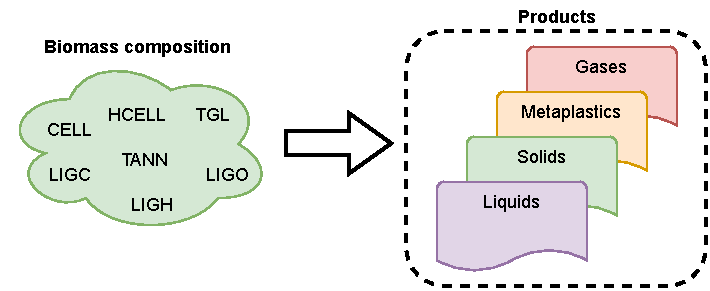
\includegraphics[width=0.7\textwidth]{figures/biocomp1.pdf}
    \caption{Seven biomass components convert to pyrolysis products according to the Debiagi et al. biomass pyrolysis kinetics scheme.}
    \label{fig:biocomp1}
\end{figure}

According to the Debiagi et al. 2015 paper \cite{Debiagi-2015}, the chemical components of the biomass are defined as shown in Table \ref{tab:chem-components}. The Debiagi paper does not provide information on how to experimentally determine these components. However, the paper provides a characterization method which estimates the biomass composition based on elemental (ultimate) analysis data. The characterization method uses the carbon (C) and hydrogen (H) content of the biomass to predict the biochemical composition in terms of cellulose, hemicellulose, lignin, tannins, and triglycerides. Splitting parameters $\alpha$, $\beta$, $\gamma$, $\delta$, and $\epsilon$ are used to improve the validity of the characterization procedure by accounting for extractives in the biomass.

\begin{table}[H]
    \centering
    \caption{Chemical components representing biomass composition needed for the Debiagi et al. pyrolysis kinetics.}
    \label{tab:chem-components}
    \begin{tabular}{lp{2cm}p{7cm}}
        \toprule
        Biomass composition & Symbol & Description \\
        \midrule
        cellulose     & CELL & glucan \\
        \addlinespace[0.2in]
        hemicellulose & GMSW XYHW XYGR & mixture of sugars such as hexoses and pentoses; mainly xylose, mannose, galactose, and arabinose \\
        \addlinespace[0.2in]
        lignin        & LIG & aromatic alcohols such as coniferyl, sinapyl, p-coumaryl alcohol\\
        \addlinespace[0.2in]
        lignin-c      & LIG-C & carbon-rich lignin \\
        \addlinespace[0.2in]
        lignin-h      & LIG-H & hydrogen-rich lignin \\
        \addlinespace[0.2in]
        lignin-o      & LIG-O & oxygen-rich lignin \\
        \addlinespace[0.2in]
        tannins       & TANN & hydrophilic extractives, phenolics, ethanol and water, represented by a gallocatechin polymer \\
        \addlinespace[0.2in]
        triglycerides & TGL & hydrophobic extractives, hexane and ether, linoleic acid \\
        \bottomrule
    \end{tabular}
\end{table}

As discussed previously, the largest differences in the chemical analysis feedstock data are for the lignin, glucan, and mannan fractions. These fractions represent the cellulose (glucan), hemicellulose (xylan, galactan, arabinan, mannan, acetyl), and total lignin components of the biomass composition. Unfortunately, the chemical analysis data does not directly relate to all the biomass components needed for the pyrolysis kinetics.

Using the C and H values from the ultimate analysis data and default values for the splitting parameters, the biomass composition is estimated using the characterization method from Debiagi et al. The estimated cellulose, hemicellulose, and total lignin (LIGC + LIGH + LIGO) values are compared to the chemical analysis data using a minimization function

\begin{equation}
    \sum (a - b)^2
\end{equation}

\noindent where $a$ is the cellulose, hemicellulose, and total lignin estimated from the characterization method and $b$ is the cellulose, hemicellulose, and lignin from the chemical analysis data. The L-BFGS-B algorithm is applied to the minimization function to generate the optimum splitting parameter values such that the cellulose, hemicellulose, and total lignin are similar to the values obtained from the chemical analysis data.

Figure \ref{fig:biocomp2} demonstrates the biomass composition procedure while Table \ref{tab:biocomp3} presents the biomass compositions for each FCIC feedstock that is suitable to use with the Debiagi et al. kinetics scheme. As seen in the table, the optimization procedure is able to determine the appropriate splitting parameters when comparing the biomass composition to chemical analysis data. The biomass composition for the bark feedstock is the only composition that does not compare within 1\% of the chemical analysis values.

\begin{figure}[H]
    \centering
    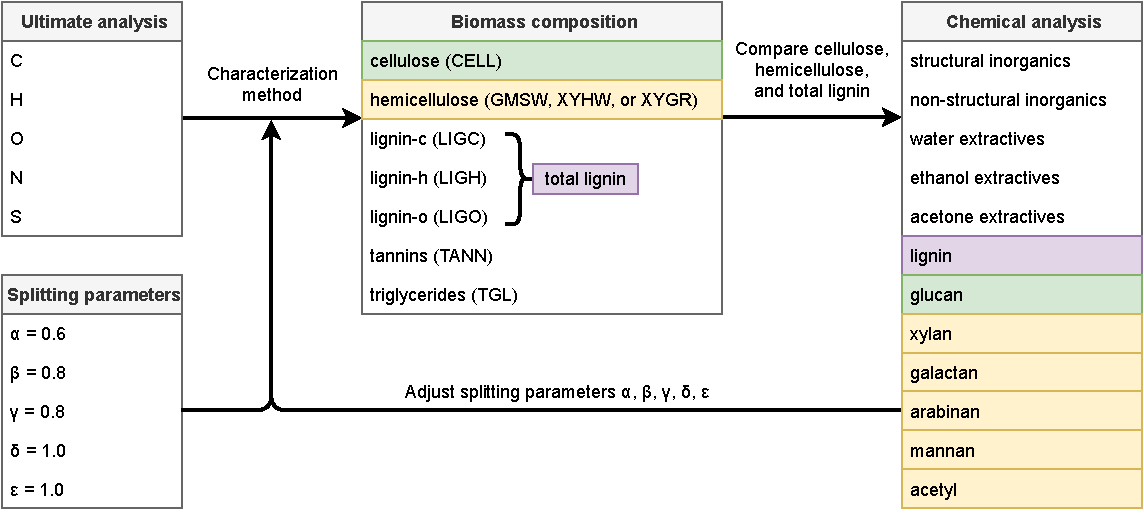
\includegraphics[width=\textwidth]{figures/biocomp2.pdf}
    \caption{Biomass composition determined from ultimate analysis data and compared with measured chemical analysis data for cellulose, hemicellulose, and total lignin.}
    \label{fig:biocomp2}
\end{figure}

\begin{longtable}{p{8cm}rr}
    \caption{Estimated biomass composition for each feedstock on a dry ash-free basis (daf). Left daf column based on chemical analysis data. Right daf column estimated from the characterization procedure using the optimized splitting parameter values.}
    \label{tab:biocomp3} \\
    \textbf{Residues, Cycle 1} & daf & daf \\
    \midrule
    cellulose       & 28.98  & 28.98 \\
    hemicellulose   & 22.02  & 22.02 \\
    lignin-c        & --     & 0.58 \\
    lignin-h        & --     & 8.79 \\
    lignin-o        & --     & 27.16 \\
    tannins         & --     & 1.60 \\
    triglycerides   & --     & 10.88 \\
    total lignin    & 36.53  & 36.53 \\
    \\
    \multicolumn{3}{l}{C = 53.31, H = 6.41} \\
    \multicolumn{3}{l}{$\alpha = 0.5175$, $\beta = 0.8996$, $\gamma = 1$, $\delta = 0.6486$, $\epsilon = 0.9246$} \\
    \\
    \textbf{Stem wood, Cycle 2} & daf & daf \\
    \midrule
    cellulose     & 39.31 & 39.91 \\
    hemicellulose & 24.84 & 25.42 \\
    lignin-c      & --    & 0.89 \\
    lignin-h      & --    & 26.20 \\
    lignin-o      & --    & 3.20 \\
    tannins       & --    & 0.01 \\
    triglycerides & --    & 4.37 \\
    total lignin  & 30.29 & 30.29 \\
    \\
    \multicolumn{3}{l}{C = 50.94, H = 6.39} \\
    \multicolumn{3}{l}{$\alpha = 0.5613$, $\beta = 0.981$, $\gamma = 0.7683$, $\delta = 0.9263$, $\epsilon = 0.9958$} \\
    \\
    \textbf{Bark, Cycle 3} & daf & daf \\
    \midrule
    cellulose     & 33.78 & 31.38 \\
    hemicellulose & 25.24 & 22.99 \\
    lignin-c      & --    & 35.14 \\
    lignin-h      & --    & 0 \\
    lignin-o      & --    & 0 \\
    tannins       & --    & 7.15 \\
    triglycerides & --    & 3.34 \\
    total lignin  & 34.29 & 35.14 \\
    \\
    \multicolumn{3}{l}{C = 55.69, H = 5.89} \\
    \multicolumn{3}{l}{$\alpha = 0.5265$, $\beta = 0.3359$, $\gamma = 0$, $\delta = 0$, $\epsilon = 0.8527$} \\
    \\
    \textbf{Needles, Cycle 4} & daf & daf \\
    \midrule
    cellulose     & 23.59 & 23.59 \\
    hemicellulose & 17.57 & 17.57 \\
    lignin-c      & --    & 0.63 \\
    lignin-h      & --    & 5.43 \\
    lignin-o      & --    & 37.30 \\
    tannins       & --    & 3.00 \\
    triglycerides & --    & 12.48 \\
    total lignin  & 43.35 & 43.35 \\
    \\
    \multicolumn{3}{l}{C = 54.71, H = 6.36} \\
    \multicolumn{3}{l}{$\alpha = 0.5225$, $\beta = 0.8364$, $\gamma = 1$, $\delta = 0.5167$, $\epsilon = 0.8996$} \\
    \\
    \textbf{Bark + needles, Cycle 5} & daf & daf \\
    \midrule
    cellulose     & 23.91 & 23.91 \\
    hemicellulose & 16.82 & 16.82 \\
    lignin-c      & --    & 6.94 \\
    lignin-h      & --    & 6.74 \\
    lignin-o      & --    & 34.53 \\
    tannins       & --    & 2.84 \\
    triglycerides & --    & 8.22 \\
    total lignin  & 48.21 & 48.21 \\
    \\
    \multicolumn{3}{l}{C = 54.79, H = 6.13} \\
    \multicolumn{3}{l}{$\alpha = 0.5366$, $\beta = 0.7312$, $\gamma = 0.7942$, $\delta = 0.6975$, $\epsilon = 0.9169$} \\
    \\
    \textbf{Residues (rep 1), Cycle 8} & daf & daf \\
    \midrule
    cellulose     & 27.44 & 27.45 \\
    hemicellulose & 20.80 & 20.81 \\
    lignin-c      & --    & 0 \\
    lignin-h      & --    & 3.71 \\
    lignin-o      & --    & 32.79 \\
    tannins       & --    & 1.98 \\
    triglycerides & --    & 13.27 \\
    total lignin  & 36.49 & 36.50 \\
    \\
    \multicolumn{3}{l}{C = 53.85, H = 6.46} \\
    \multicolumn{3}{l}{$\alpha = 0.5181$, $\beta = 1$, $\gamma = 1$, $\delta = 0.365$, $\epsilon = 0.9228$} \\
    \\
    \textbf{Residues:bark:needles 1:1:1, Cycle 10} & daf & daf \\
    \midrule
    cellulose     & 24.05 & 24.05 \\
    hemicellulose & 18.62 & 18.62 \\
    lignin-c      & --    & 7.27 \\
    lignin-h      & --    & 3.93 \\
    lignin-o      & --    & 32.08 \\
    tannins       & --    & 3.89 \\
    triglycerides & --    & 10.16 \\
    total lignin  & 43.28 & 43.28 \\
    \\
    \multicolumn{3}{l}{C = 54.91, H = 6.22} \\
    \multicolumn{3}{l}{$\alpha = 0.5128$, $\beta = 0.6851$, $\gamma = 0.7597$, $\delta = 0.5375$, $\epsilon = 0.8866$} \\
    \\
    \textbf{Residues:bark:needles 1:2:2, Cycle 11} & daf & daf \\
    \midrule
    cellulose     & 23.98 & 23.99 \\
    hemicellulose & 17.43 & 17.43 \\
    lignin-c      & --    & 10.51 \\
    lignin-h      & --    & 3.27 \\
    lignin-o      & --    & 31.12 \\
    tannins       & --    & 4.59 \\
    triglycerides & --    & 9.10 \\
    total lignin  & 44.89 & 44.89 \\
    \\
    \multicolumn{3}{l}{C = 55.25, H = 6.14} \\
    \multicolumn{3}{l}{$\alpha = 0.5285$, $\beta = 0.6664$, $\gamma = 0.6661$, $\delta = 0.5255$, $\epsilon = 0.88$} \\
    \\
    \textbf{Air classified (10 Hz), Cycle 12} & daf & daf \\
    \midrule
    cellulose     & 32.44 & 32.44 \\
    hemicellulose & 24.13 & 24.13 \\
    lignin-c      & --    & 4.82 \\
    lignin-h      & --    & 13.86 \\
    lignin-o      & --    & 16.93 \\
    tannins       & --    & 0 \\
    triglycerides & --    & 7.83 \\
    total lignin  & 35.60 & 35.60 \\
    \\
    \multicolumn{3}{l}{C = 52.74, H = 6.37} \\
    \multicolumn{3}{l}{$\alpha = 0.5228$, $\beta = 0.7661$, $\gamma = 0.8174$, $\delta = 0.8261$, $\epsilon = 1$} \\
    \\
    \textbf{Air classified (28 Hz), Cycle 13} & daf & daf \\
    \midrule
    cellulose     & 34.37 & 34.37 \\
    hemicellulose & 25.94 & 25.94 \\
    lignin-c      & --    & 3.76 \\
    lignin-h      & --    & 18.38 \\
    lignin-o      & --    & 13.09 \\
    tannins       & --    & 0 \\
    triglycerides & --    & 4.46 \\
    total lignin  & 35.23 & 35.23 \\
    \\
    \multicolumn{3}{l}{C = 51.67, H = 6.26} \\
    \multicolumn{3}{l}{$\alpha = 0.5191$, $\beta = 0.8365$, $\gamma = 0.8302$, $\delta = 0.9101$, $\epsilon = 0.9996$} \\
    \\
    \textbf{Whole tree (13 yr), Cycle 15} & daf & daf \\
    \midrule
    cellulose     & 34.12 & 34.13 \\
    hemicellulose & 25.50 & 25.50 \\
    lignin-c      & --    & 0.91 \\
    lignin-h      & --    & 16.12 \\
    lignin-o      & --    & 16.60 \\
    tannins       & --    & 0.66 \\
    triglycerides & --    & 6.08 \\
    total lignin  & 33.63 & 33.63 \\
    \\
    \multicolumn{3}{l}{C = 51.63, H = 6.31} \\
    \multicolumn{3}{l}{$\alpha = 0.5216$, $\beta = 1$, $\gamma = 0.9175$, $\delta = 0.845$, $\epsilon = 0.9517$} \\
    \\
    \textbf{Stem wood (13 yr), Cycle 16} & daf & daf \\
    \midrule
    cellulose     & 37.46 & 37.46 \\
    hemicellulose & 26.14 & 26.14 \\
    lignin-c      & --    & 1.84 \\
    lignin-h      & --    & 24.58 \\
    lignin-o      & --    & 6.38 \\
    tannins       & --    & 0.01 \\
    triglycerides & --    & 3.59 \\
    total lignin  & 32.80 & 32.80 \\
    \\
    \multicolumn{3}{l}{C = 51.07, H = 6.31} \\
    \multicolumn{3}{l}{$\alpha = 0.5387$, $\beta = 0.9443$, $\gamma = 0.7995$, $\delta = 0.9372$, $\epsilon = 0.9991$} \\
\end{longtable}

\subsection{Batch reactor model}

The material balance for a typical chemical reactor is shown in Equation \ref{eq:typical-balance} where $C_0$ is inlet concentration, $C$ is outlet concentration, $v$ is volumetric flow rate, $r$ is the reaction rate, and $V$ is the reactor volume.

\begin{equation}
    \label{eq:typical-balance}
    \begin{aligned}
        accumulation &= input - output + reaction \\
        \frac{dC}{dt} V &= v C_0 - v C + r V
    \end{aligned}
\end{equation}

A batch reactor was modeled to understand the time scales associated with the biomass pyrolysis kinetics. For the batch reactor, input and output is zero therefore only the accumulation and reaction terms remain in the material balance. For a constant volume reactor the $V$ terms cancel out; therefore, Equation \ref{eq:batch-balance} represents the material balance for a batch reactor model. A depiction of a batch reactor can be seen in Figure \ref{fig:batch-reactor}. The Cantera Python package was used to model the batch reactor as an IdealGasReactor \cite{Cantera-2018}.

\begin{equation}
    \label{eq:batch-balance}
    \begin{aligned}
        accumulation &= 0 - 0 + reaction \\
        \frac{dC}{dt} &= r
    \end{aligned}
\end{equation}

\begin{figure}[H]
    \centering
    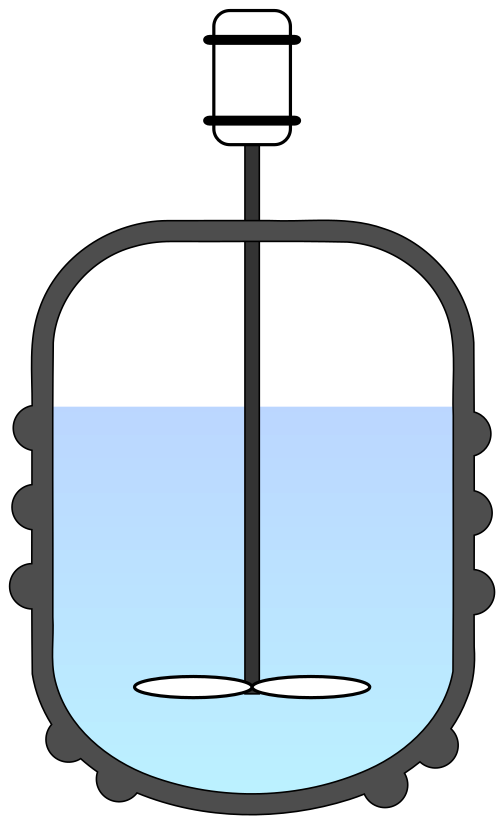
\includegraphics[width=0.2\textwidth]{figures/batch-reactor.png}
    \caption{Representation of a batch reactor system. Source: Wikipedia.}
    \label{fig:batch-reactor}
\end{figure}

Reaction rates in the batch reactor model are determined from a forward rate constant $k$ based on an Arrhenius function

\begin{equation}
    k = A\,T^b e^{-E / RT}
\end{equation}

\noindent where $A$ is the pre-exponential factor, $T$ is the reaction temperature, $b$ is the temperature exponent, $E$ is the activation energy, and $R$ is the universal gas constant.

\subsection{CSTR series model}

The material balance associated with a continuous stirred tank reactor (CSTR) model for an example chemical $A$ is

\begin{equation}
    \begin{aligned}
        accumulation &= input - output + reaction \\
        0 &= input - output + reaction \\
        0 &= v C_{A0} - v C_A + r_A V \\
        C_A &= C_{A0} + r_A\;\tau
    \end{aligned}
\end{equation}

\noindent where $v$ is the volumetric flow rate (m$^3$/s), $C_{A0}$ is the inlet concentration (mol/m$^3$), $C_A$ is the outlet concentration (mol/m$^3$), $r_A$ is the reaction rate (mol/m$^3$s), $V$ is the reactor volume (m$^3$), and $\tau$ is the residence time (s) of chemical $A$ in the reactor.

\section{Results and discussion}

Here.

\section{Conclusions}

Here.

\section{Hardware requirements}

The reduced order models discussed in this report were developed and executed on a MacBook Pro laptop (see hardware specs below). The models do not give as much detail as full 3D simulations but they provide good enough results in a timely manner; as such, they lend themselves well to process modeling, design of experiments, and rapid prototyping tasks.

\begin{itemize}
    \item MacBook Pro, 16-inch, 2019 model
    \item 2.3 GHz 8-core Intel i9 CPU
    \item 32 GB 2667 MHz DDR4 memory
    \item 4 GB AMD Radeon Pro 5500M GPU
    \item macOS Big Sur version 11.6
\end{itemize}

\section{Source code}

Source code for this project is available on GitHub at the link provided below. See the README markdown document in the repository for more information.

\begin{itemize}
    \item \url{https://github.com/wigging/fcic-pyrolysis}
\end{itemize}

% --- References -------------------------------------------------------------

\printbibliography

\end{document}